\documentclass[conference]{IEEEtran}

\usepackage{cite}
\usepackage{amsmath,amssymb,amsfonts}
\usepackage{graphicx}
\usepackage{textcomp}
\usepackage{xcolor}
\usepackage{booktabs}
\usepackage{multirow}
\usepackage{url}
\usepackage[caption=false]{subfig}
\usepackage{listings}
\usepackage{tikz}
\usetikzlibrary{arrows.meta,positioning,decorations.pathreplacing}

\begin{document}

\title{QCV: When AI Reads Quantum --- Toward AlphaFold for Quantum Circuit Discovery}

\author{
\IEEEauthorblockN{Dongping Liu}
\IEEEauthorblockA{Tenorshare (Hong Kong) Limited\\Hong Kong, China\\steven.dpliu@gmail.com}
\and
\IEEEauthorblockN{Aoyu Zhang}
\IEEEauthorblockA{Amazon Web Services\\Beijing, China\\aoyuzhan@amazon.com}
\and
\IEEEauthorblockN{Luyao Zhang}
\IEEEauthorblockA{Duke Kunshan University\\Suzhou, China\\lz183@duke.edu}
}

\maketitle

\begin{abstract}
Can AI learn to read quantum circuit diagrams---and eventually discover new ones? Inspired by AlphaFold's transformation of structural biology, we take the first step toward AI-driven quantum circuit discovery by establishing QCV-Dataset: the first multimodal quantum circuit dataset comprising 132 circuits across 13 categories (1--10 qubits) with seven modalities per circuit---diagram images, dual-SDK executable code (Amazon Braket and Qiskit), simulation results, bilingual annotations, natural language target descriptions, and optimization equivalence pairs. Evaluating three multimodal large language models under Basic Vision (BV) and Thinking Vision (TV) prompting, we demonstrate that AI can already reliably interpret quantum circuits (97.0\% accuracy for the strongest model). More importantly, we discover a \emph{CoT sensitivity window}---a fundamental principle showing that chain-of-thought reasoning only impacts performance near a model's capability boundary, helping weaker models (+20pp) but degrading advanced performance ($-$17pp), while leaving mid-tier models entirely unaffected. This finding, absent in classical circuit experiments, reveals something deeper about how AI reasons about quantum structures. We validate on 31 blockchain-relevant circuits spanning quantum threats to Bitcoin (Shor vs.\ ECDSA, Grover vs.\ SHA-256), post-quantum defenses (Kyber, Dilithium, SPHINCS+), and quantum infrastructure---finding that structural regularity, not qubit count, determines comprehension success. Dataset and code: \url{https://github.com/QuantBlockchain/quantum-circuit-vision}.
\end{abstract}

\section{Introduction}

The year 2025 marked a quantum inflection point: the Nobel Prize in Physics recognized experiments with superconducting qubits that enabled macroscopic quantum coherence, while the ACM Turing Award honored the foundations of quantum information theory---including the BB84 protocol that underpins quantum key distribution. The United Nations declared 2025 the International Year of Quantum Science and Technology. Quantum computing has crossed from theoretical promise to engineering reality.

Yet a fundamental bottleneck persists: the gap between how quantum algorithms are \emph{communicated} (as circuit diagrams in papers, textbooks, and courses) and how they are \emph{executed} (as code in SDKs such as Amazon Braket~\cite{braket}, Qiskit~\cite{qiskit}, or Cirq). Every quantum circuit published in a research paper must be manually translated into executable code---a tedious, error-prone process requiring both visual interpretation skills and SDK-specific programming expertise. As quantum hardware scales and the volume of published circuits grows exponentially, this manual translation becomes an unsustainable bottleneck for scientific progress.

We argue that \textbf{automating the translation from quantum circuit diagrams to verified executable code is a foundational AI-for-Science challenge}---analogous to how AlphaFold~\cite{jumper2021alphafold} automated protein structure prediction from amino acid sequences. Just as AlphaFold accelerated structural biology by orders of magnitude, a system that reliably reads quantum circuit diagrams and produces verified code could accelerate quantum algorithm development, quantum-safe cryptography research~\cite{fedorov2018quantum,liu2026quantumsafe}, and the broader quantum computing ecosystem.

This challenge is particularly urgent for blockchain security. As platforms migrate to post-quantum cryptography, researchers publish PQC circuit designs that must be rapidly prototyped and verified. Shor's algorithm threatens ECDSA signatures protecting billions in Bitcoin assets; Grover's algorithm offers quadratic speedup against SHA-256 mining. The ability to instantly translate these threat-model circuits from diagrams to executable code---and verify their correctness---is critical infrastructure for the quantum-safe transition.

In this paper, we take the first step toward this vision by establishing QCV-Dataset---the first multimodal quantum circuit dataset---and the evaluation methodology and baseline results that future circuit-discovery systems will build upon.

Recent work has demonstrated that large language models (LLMs) can assist in hardware design automation. Projects such as ChipChat~\cite{blocklove2023chipchat}, VeriGen~\cite{thakur2023verigen}, GPT4AIGChip~\cite{fu2023gpt4aigchip}, ChipNemo~\cite{liu2023chipnemo}, and ChatEDA~\cite{he2023chateda} have explored using LLMs to generate HDL code, EDA scripts, and accelerator designs from textual specifications. Multimodal models such as GPT-4~\cite{openai2023gpt4} and LLaVA~\cite{liu2023llava} have further demonstrated strong visual reasoning capabilities across domains including mathematical problem solving~\cite{lu2023mathvista}. Our prior work, VGV~\cite{wong2024vgv}, extended this line of research to the visual domain, showing that MMLLMs can generate Verilog code from classical circuit diagrams. VGV introduced the Thinking Vision (TV) prompting method, which improved open-source model performance by over 50\% compared to Basic Vision (BV).

Quantum circuit diagrams possess several properties that make them particularly amenable to visual code generation by MMLLMs. First, quantum gate symbols follow standardized conventions (e.g., $H$ for Hadamard, $\oplus$ for CNOT targets, $\bullet$ for control qubits), unlike classical microarchitecture diagrams which lack industry-wide standardization. Second, quantum circuits have a strictly left-to-right temporal structure with no feedback loops. Third, the gate vocabulary is finite and well-defined. These properties suggest that MMLLMs may achieve higher accuracy on quantum circuits than on classical ones.

In this paper, we present QCV (Quantum Circuit Vision), the first systematic study of MMLLM-based code generation from quantum circuit diagram images, accompanied by QCV-Dataset, the first multimodal quantum circuit dataset. Our contributions are:
\begin{enumerate}
    \item We construct QCV-Dataset: 132 quantum circuits across 13 categories (1--10 qubits) with seven modalities per circuit---diagram images, executable code in two SDKs (Braket and Qiskit), simulation results, bilingual annotations, natural language target descriptions, and optimization equivalence pairs---publicly released for community use.
    \item We evaluate three MMLLMs (Claude Opus 4.6, Sonnet 4.6, and Haiku 4.5) under BV and TV visual modes on 21 circuits, discovering a \emph{CoT sensitivity window}: TV's effect depends on model capability level, a finding not observed in prior classical circuit experiments.
    \item We propose an end-to-end verification pipeline using unitary matrix fidelity on Amazon Braket's LocalSimulator, and validate on 31 blockchain-relevant circuits covering quantum threats, post-quantum defenses, and quantum infrastructure.
    \item We release all code, data, and annotations at \url{https://github.com/QuantBlockchain/quantum-circuit-vision} to enable reproducibility and future research toward AI-driven quantum circuit discovery.
\end{enumerate}

Our results show that Claude Opus 4.6 under BV achieves a weighted score of 97.0\%, passing 20 out of 21 circuits, Sonnet 4.6 scores 88.5\%, and Haiku 4.5 scores 46.5\%. The performance gap between models widens with circuit complexity (40pp between Opus and Haiku at Basic, 67pp at Advanced), indicating that advanced visual reasoning capabilities are critical for complex quantum circuit understanding.

\section{QCV-Dataset}

\begin{figure*}[t]
\centering
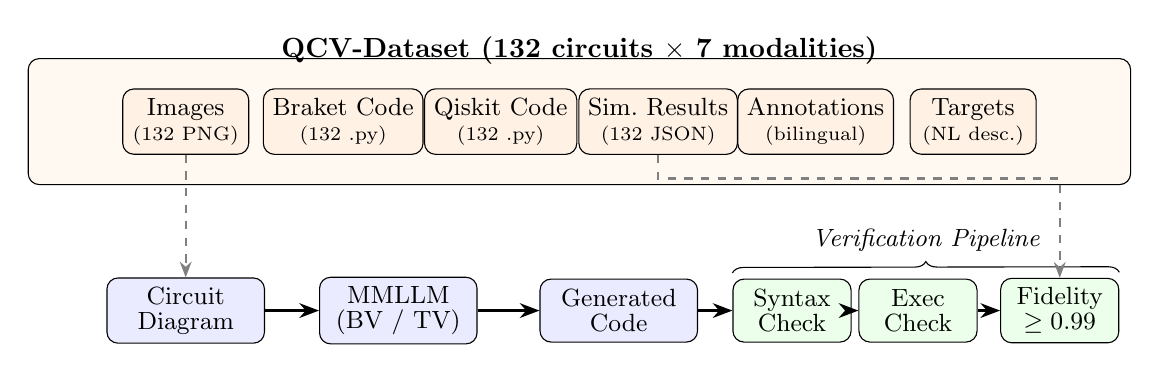
\begin{tikzpicture}[node distance=0.5cm, every node/.style={font=\small},
  dbox/.style={draw, rounded corners, minimum height=0.7cm, minimum width=1.6cm, align=center, fill=orange!10},
  box/.style={draw, rounded corners, minimum height=0.8cm, minimum width=2.0cm, align=center, fill=blue!8},
  vbox/.style={draw, rounded corners, minimum height=0.8cm, minimum width=1.5cm, align=center, fill=green!8},
  arr/.style={-{Stealth[length=2.5mm]}, thick},
  darr/.style={-{Stealth[length=2mm]}, thick, dashed, gray}]
% Dataset layer
\node[draw, rounded corners, fill=orange!5, minimum width=14.0cm, minimum height=1.6cm] (dataset) at (6.5,3.2) {};
\node[font=\normalsize\bfseries] at (6.5,4.1) {QCV-Dataset (132 circuits $\times$ 7 modalities)};
\node[dbox] (d1) at (1.5,3.2) {Images\\[-2pt]\scriptsize(132 PNG)};
\node[dbox] (d2) at (3.5,3.2) {Braket Code\\[-2pt]\scriptsize(132 .py)};
\node[dbox] (d3) at (5.5,3.2) {Qiskit Code\\[-2pt]\scriptsize(132 .py)};
\node[dbox] (d4) at (7.5,3.2) {Sim.\ Results\\[-2pt]\scriptsize(132 JSON)};
\node[dbox] (d5) at (9.5,3.2) {Annotations\\[-2pt]\scriptsize(bilingual)};
\node[dbox] (d6) at (11.5,3.2) {Targets\\[-2pt]\scriptsize(NL desc.)};
% Evaluation pipeline
\node[box] (img) at (1.5,0.8) {Circuit\\[-2pt]Diagram};
\node[box] (llm) at (4.2,0.8) {MMLLM\\[-2pt](BV / TV)};
\node[box] (code) at (7.0,0.8) {Generated\\[-2pt]Code};
\node[vbox] (syn) at (9.2,0.8) {Syntax\\[-2pt]Check};
\node[vbox] (exe) at (10.8,0.8) {Exec\\[-2pt]Check};
\node[vbox] (fid) at (12.6,0.8) {Fidelity\\[-2pt]$\geq 0.99$};
\draw[arr] (img) -- (llm);
\draw[arr] (llm) -- (code);
\draw[arr] (code) -- (syn);
\draw[arr] (syn) -- (exe);
\draw[arr] (exe) -- (fid);
% Brace for verification
\draw[decorate, decoration={brace, amplitude=4pt, raise=2pt}] (syn.north west) -- (fid.north east) node[midway, above=6pt, font=\small\itshape] {Verification Pipeline};
% Connections from dataset
\draw[darr] (d1.south) -- ++(0,-0.6) -| (img.north);
\draw[darr] (d4.south) -- ++(0,-0.3) -| (fid.north);
\end{tikzpicture}
\caption{QCV system overview. \textbf{Top:} QCV-Dataset provides 132 quantum circuits with 7 data modalities---circuit images, executable code in two SDKs (Braket and Qiskit), simulation results, bilingual annotations, natural language target descriptions, and optimization equivalence pairs. \textbf{Bottom:} The evaluation pipeline processes a circuit diagram image through an MMLLM under BV or TV mode, then verifies the generated code through syntax checking, execution, and unitary matrix fidelity ($F \geq 0.99$).}
\label{fig:workflow}
\end{figure*}

Following the approach established in VGV~\cite{wong2024vgv}, we design a difficulty-graded benchmark, define two visual prompting modes, and build an end-to-end verification pipeline tailored to quantum circuits.

\subsection{Benchmark Design}

We construct QCV-Dataset, a multimodal quantum circuit dataset of 132 circuits across 13 categories, with seven data modalities per circuit. For the evaluation reported in this paper, we select a representative subset of 21 circuits across three difficulty levels, inspired by standard quantum computing curricula~\cite{nielsen2010quantum}. All circuit diagrams are generated programmatically using Qiskit's \texttt{matplotlib} drawer~\cite{qiskit}, ensuring reproducible and unambiguous visual inputs. Ground truth implementations are provided in both Amazon Braket SDK~\cite{braket} and Qiskit.

The full dataset spans 13 categories: basic gates (5), intermediate algorithms (10), advanced algorithms (6), blockchain protocols (11), gate-type coverage (15), qubit scaling 4--10q (12), classical algorithms (15), variational circuits (10), error correction codes (8), quantum ML (10), blockchain extended (8), visual variants (10), and BTC/blockchain quantum security (12). The 21 evaluated circuits are drawn from the first three categories:

\begin{itemize}
    \item \textbf{Basic (5 circuits):} Single-gate or single-entangling-gate circuits testing fundamental gate recognition (Hadamard, CNOT, Bell state, GHZ state, Toffoli).
    \item \textbf{Intermediate (10 circuits):} Multi-gate circuits requiring understanding of gate composition, control relationships, and parameterized rotations (SWAP decomposition, 2-qubit QFT, teleportation, Deutsch, superdense coding, Grover 2-qubit, parameterized rotation, Fredkin, shift register, phase estimation).
    \item \textbf{Advanced (6 circuits):} Complete quantum algorithms involving complex multi-qubit structures (3-qubit QFT, 3-qubit Grover, VQE ansatz, QAOA, quantum walk, Bernstein-Vazirani).
\end{itemize}

Each circuit in the full dataset includes: (1)~a PNG diagram image, (2)~executable Braket SDK code, (3)~executable Qiskit code, (4)~simulation results (state vectors from LocalSimulator), (5)~structured bilingual annotations (English/Chinese), (6)~a natural language target description for circuit synthesis tasks, and (7)~optimization equivalence pairs where applicable. Additionally, 27 annotated failure cases from our MMLLM experiments are included for error analysis research. Table~\ref{tab:dataset} summarizes the 13 categories, and Table~\ref{tab:benchmark} lists the 21 evaluated circuits.

\begin{table}[t]
\centering
\caption{QCV-Dataset: 132 Circuits across 13 Categories}
\label{tab:dataset}
\small
\begin{tabular}{@{}llcc@{}}
\toprule
Category & Focus & Count & Qubits \\
\midrule
Basic (demo) & Fundamental gates & 5 & 1--3 \\
Intermediate (inter) & Multi-gate composition & 10 & 2--4 \\
Advanced (adv) & Complete algorithms & 6 & 3--5 \\
Blockchain & Quantum protocols & 11 & 2--8 \\
\midrule
A: Gate Coverage & All standard gate types & 15 & 1--3 \\
B: Qubit Scaling & 4--10 qubit circuits & 12 & 4--10 \\
C: Classical Algorithms & Textbook algorithms & 15 & 2--4 \\
D: Variational & NISQ-era ans\"{a}tze & 10 & 2--4 \\
E: Error Correction & QEC codes & 8 & 3--9 \\
F: Quantum ML & QNN, QCNN, kernels & 10 & 2--8 \\
G: Blockchain Ext. & Crypto protocols & 8 & 3--6 \\
H: Visual Variants & Layout robustness & 10 & 2--4 \\
I: BTC Security & Threats \& PQC defense & 12 & 4--7 \\
\midrule
\multicolumn{2}{l}{\textbf{Total}} & \textbf{132} & \textbf{1--10} \\
\bottomrule
\end{tabular}
\end{table}

\begin{table}[t]
\centering
\caption{Evaluated Subset: 21 Quantum Circuits}
\label{tab:benchmark}
\small
\begin{tabular}{@{}clll@{}}
\toprule
No. & Difficulty & Circuit & Qubits \\
\midrule
1  & Basic & Hadamard          & 1 \\
2  & Basic & CNOT              & 2 \\
3  & Basic & Bell State        & 2 \\
4  & Basic & GHZ State         & 3 \\
5  & Basic & Toffoli (CCX)     & 3 \\
\midrule
6  & Intermediate & SWAP Decomposition    & 2 \\
7  & Intermediate & 2-Qubit QFT           & 2 \\
8  & Intermediate & Teleportation Prep    & 3 \\
9  & Intermediate & Deutsch Algorithm     & 2 \\
10 & Intermediate & Superdense Coding     & 2 \\
11 & Intermediate & 2-Qubit Grover        & 2 \\
12 & Intermediate & Parameterized Rotation & 2 \\
13 & Intermediate & Fredkin (CSWAP)       & 3 \\
14 & Intermediate & Shift Register        & 4 \\
15 & Intermediate & Phase Estimation      & 3 \\
\midrule
16 & Advanced & 3-Qubit QFT            & 3 \\
17 & Advanced & 3-Qubit Grover         & 3 \\
18 & Advanced & VQE Ansatz             & 4 \\
19 & Advanced & QAOA (MaxCut)          & 4 \\
20 & Advanced & Quantum Walk           & 4 \\
21 & Advanced & Bernstein-Vazirani     & 5 \\
\bottomrule
\end{tabular}
\end{table}

\section{Evaluation Methodology}

\subsection{Visual Modes}

We evaluate two visual prompting strategies adapted from VGV~\cite{wong2024vgv}:

\textbf{Basic Vision (BV)} provides the circuit diagram image with a direct code generation instruction:

\smallskip
\noindent\fbox{\parbox{0.93\columnwidth}{\small\textit{``Please generate Amazon Braket SDK Python code based on this quantum circuit diagram. Requirements: use \texttt{from braket.circuits import Circuit}; output only complete executable Python code; no explanation, no markdown.''}}}
\smallskip

\textbf{Thinking Vision (TV)} adds a chain-of-thought analysis step before code generation:

\smallskip
\noindent\fbox{\parbox{0.93\columnwidth}{\small\textit{``Please first analyze this quantum circuit diagram: 1.~How many qubit lines? What are their labels? 2.~What gates appear from left to right? 3.~Which gates have control qubits? Which line is control, which is target? Then generate Amazon Braket SDK Python code based on your analysis.''}}}
\smallskip

Unlike VGV, which also varied prompt detail levels (Short/Medium/High), we use a single prompt per mode to isolate the effect of chain-of-thought reasoning from prompt informativeness.

\begin{figure*}[t]
\centering
\subfloat[Basic: Bell State (2q, 2 gates) --- trivial for AI]{
\includegraphics[width=0.18\textwidth]{figures/demo_03_bell.pdf}}
\hfill
\subfloat[Intermediate: 2-Qubit Grover (2q, 9 gates)]{
\includegraphics[width=0.25\textwidth]{figures/inter_06_grover2.pdf}}
\hfill
\subfloat[Advanced: QAOA MaxCut (4q, 16 gates) --- all models struggle]{
\includegraphics[width=0.28\textwidth]{figures/adv_04_qaoa.pdf}}
\hfill
\subfloat[Blockchain: 8-Qubit Consensus (8q, 20 gates) --- passes due to regularity]{
\includegraphics[width=0.25\textwidth]{figures/blockchain_consensus.pdf}}
\caption{Representative circuits spanning the difficulty spectrum. Notably, the 8-qubit consensus circuit (d) passes with perfect fidelity due to its regular repeating structure, while the 4-qubit QAOA (c) fails for multiple models due to parallel gate layers---demonstrating that structural regularity, not qubit count, determines AI comprehension success.}
\label{fig:circuits}
\end{figure*}

\subsection{Verification Pipeline}

Generated code is verified through a three-level pipeline:

\begin{enumerate}
    \item \textbf{Syntax check:} The extracted Python code is compiled using \texttt{compile()} to detect syntax errors.
    \item \textbf{Execution check:} The code is executed in a sandboxed namespace. We verify that a valid Braket \texttt{Circuit} object is produced.
    \item \textbf{Unitary fidelity check:} We compute the full unitary matrix of both the generated circuit and the ground truth by running each computational basis state on Amazon Braket's LocalSimulator~\cite{braket} with \texttt{shots=0}. The fidelity is computed as $F = |\mathrm{Tr}(U_{\text{gt}}^\dagger U_{\text{gen}})| / d$, where $d = 2^n$ is the Hilbert space dimension. A circuit passes if $F \geq 0.99$.
\end{enumerate}

This unitary-based verification is more rigorous than state-vector comparison on a single input, as it checks correctness across all possible input states. It is also phase-tolerant, correctly handling circuits that differ only by a global phase.

\subsection{Evaluation Metrics}

We report two metrics following VGV~\cite{wong2024vgv}:

\textbf{Pass rate} is the fraction of circuits for which the generated code passes all three verification levels, reported per difficulty level.

\textbf{Weighted score} aggregates pass rates across difficulty levels: $S = 0.2 \times R_{\text{Basic}} + 0.3 \times R_{\text{Intermediate}} + 0.5 \times R_{\text{Advanced}}$, where $R$ denotes the pass rate at each level. The weights reflect increasing difficulty, with Advanced circuits contributing the most to the overall score.

\section{Results and Scientific Findings}

\subsection{Experimental Setup}

We evaluate three MMLLMs from the Claude family, spanning high-end, mid-tier, and lightweight capability levels (Table~\ref{tab:models}). All models are accessed through a unified command-line interface (\texttt{kiro-cli}) in non-interactive mode, ensuring identical execution conditions. Each circuit diagram is provided as a PNG image alongside the BV or TV prompt. The total experiment comprises 21 circuits $\times$ 3 models $\times$ 2 visual modes = 126 invocations.

\begin{table}[t]
\centering
\caption{Evaluated MMLLMs}
\label{tab:models}
\small
\begin{tabular}{@{}lll@{}}
\toprule
Model & Tier & Relative Cost \\
\midrule
Claude Opus 4.6   & High-end    & 2.20$\times$ \\
Claude Sonnet 4.6 & Mid-tier    & 1.30$\times$ \\
Claude Haiku 4.5  & Lightweight & 0.40$\times$ \\
\bottomrule
\end{tabular}
\end{table}

All generated code is verified on Amazon Braket's LocalSimulator (a free, local state-vector simulator) using the unitary fidelity pipeline described in Section~II-C. No cloud quantum hardware is used.

\subsection{Results}

Table~\ref{tab:results} presents the complete pass rate matrix across models, visual modes, and difficulty levels.

\begin{table}[t]
\centering
\caption{Pass Rates by Model, Visual Mode, and Difficulty}
\label{tab:results}
\footnotesize
\begin{tabular}{@{}ll ccc c@{}}
\toprule
 & & \multicolumn{3}{c}{Pass Rate} & Wtd. \\
\cmidrule(lr){3-5}
Model & Mode & Bas. & Int. & Adv. & Score \\
\midrule
\multirow{2}{*}{Opus}
  & BV & 5/5\,(100\%) & 9/10\,(90\%)  & 6/6\,(100\%) & \textbf{97.0\%} \\
  & TV & 5/5\,(100\%) & 10/10\,(100\%) & 5/6\,(83\%)  & 91.5\% \\
\midrule
\multirow{2}{*}{Sonnet}
  & BV & 5/5\,(100\%) & 9/10\,(90\%)  & 5/6\,(83\%)  & 88.5\% \\
  & TV & 5/5\,(100\%) & 9/10\,(90\%)  & 5/6\,(83\%)  & 88.5\% \\
\midrule
\multirow{2}{*}{Haiku}
  & BV & 3/5\,(60\%)  & 6/10\,(60\%)  & 2/6\,(33\%)  & 46.5\% \\
  & TV & 4/5\,(80\%)  & 7/10\,(70\%)  & 1/6\,(16\%)  & 45.0\% \\
\bottomrule
\end{tabular}
\end{table}

Opus 4.6 under BV achieves the highest weighted score (97.0\%), passing 20 of 21 circuits. Its sole failure is an API naming error (\texttt{.crz()} instead of \texttt{.cphaseshift()}) on the phase estimation circuit. Under TV, Opus achieves a perfect 10/10 on Intermediate but drops to 5/6 on Advanced due to an incorrect QAOA implementation (fidelity = 0.25).

Sonnet 4.6 scores 88.5\% under both BV and TV---identical results across all difficulty levels. It fails on phase estimation (BV: structural error with fidelity 0.23; TV: API error using \texttt{.crz()}) and QAOA (BV: fidelity 0.50; TV: fidelity 0.15) under both modes, though with different failure mechanisms.

Haiku 4.5 scores substantially lower across all conditions. Under BV, it passes 11 of 21 circuits; under TV, 12 of 21. Its weighted scores (46.5\% BV, 45.0\% TV) are roughly half of Opus's, with the gap widening at higher difficulty levels. Note that the weighted scores differ substantially from raw pass rates (e.g., 11/21 = 52\% raw vs.\ 46.5\% weighted) because Advanced circuits carry 50\% of the weight.


\subsection{Finding 1: CoT Sensitivity Window}

\begin{figure}[t]
\centering
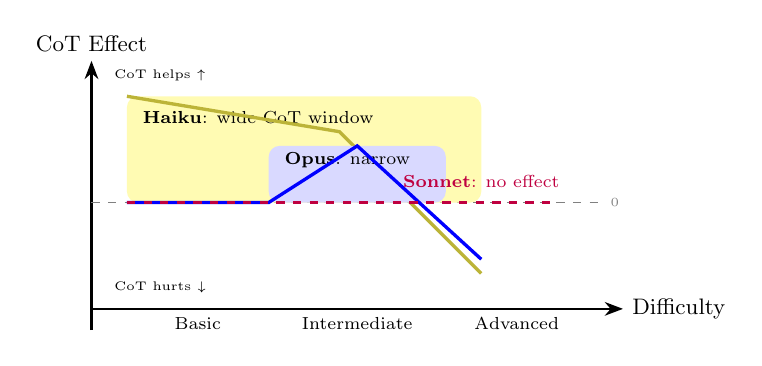
\begin{tikzpicture}[every node/.style={font=\small}, scale=0.9, transform shape]
% Axis
\draw[-{Stealth}, thick] (0,0) -- (7.5,0) node[right] {\small Difficulty};
\draw[-{Stealth}, thick] (0,-0.3) -- (0,3.5) node[above] {\small CoT Effect};
% Difficulty labels
\node[below, font=\scriptsize] at (1.5,0) {Basic};
\node[below, font=\scriptsize] at (3.75,0) {Intermediate};
\node[below, font=\scriptsize] at (6.0,0) {Advanced};
% Zero line
\draw[dashed, gray] (0,1.5) -- (7.2,1.5) node[right, font=\tiny, gray] {0};
% Haiku (wide window)
\fill[yellow!30, rounded corners] (0.5,1.5) rectangle (5.5,3.0);
\node[font=\scriptsize, anchor=west] at (0.6,2.7) {\textbf{Haiku}: wide CoT window};
\draw[yellow!70!black, very thick] (0.5,3.0) -- (3.5,2.5) -- (5.5,0.5);
% Opus (narrow window)
\fill[blue!15, rounded corners] (2.5,1.5) rectangle (5.0,2.3);
\node[font=\scriptsize, anchor=west] at (2.6,2.1) {\textbf{Opus}: narrow};
\draw[blue, very thick] (0.5,1.5) -- (2.5,1.5) -- (3.75,2.3) -- (5.5,0.7);
% Sonnet (no window)
\draw[purple, very thick, dashed] (0.5,1.5) -- (6.5,1.5);
\node[font=\scriptsize, purple] at (5.5,1.8) {\textbf{Sonnet}: no effect};
% Annotations
\node[font=\tiny, anchor=west] at (0.2,3.3) {CoT helps $\uparrow$};
\node[font=\tiny, anchor=west] at (0.2,0.3) {CoT hurts $\downarrow$};
\end{tikzpicture}
\caption{The CoT Sensitivity Window: chain-of-thought prompting only helps near a model's capability boundary. Haiku has a wide window (CoT helps on Basic/Intermediate), Opus has a narrow window (only Intermediate), and Sonnet has no window (CoT has zero effect at all levels).}
\label{fig:cot_concept}
\end{figure}

The most notable finding is that TV's effect depends not only on circuit complexity but also on model capability level (Fig.~\ref{fig:cot_concept}, Fig.~\ref{fig:cot_reversal}):

\textbf{Haiku (weak):} TV has a strong positive effect on simpler circuits that diminishes and reverses with complexity. Basic: +20pp (TV helps select correct API, e.g., \texttt{.ccnot()} instead of \texttt{.toffoli()}). Intermediate: +10pp. Advanced: $-$17pp.

\textbf{Opus (strong):} TV has a moderate positive effect on intermediate circuits but reverses on advanced ones. Basic: 0pp (already at ceiling). Intermediate: +10pp. Advanced: $-$17pp.

\textbf{Sonnet (mid-tier):} TV has \emph{zero effect} at all difficulty levels. BV and TV produce identical pass rates (100\%/90\%/83\%). Notably, Sonnet fails on the same circuits (phase estimation, QAOA) under both modes but through different mechanisms---BV produces a structural error (fidelity 0.23) on phase estimation while TV produces an API error (\texttt{.crz()}), indicating that TV alters the reasoning pathway without changing the outcome.

\begin{figure}[t]
\centering
\includegraphics[width=0.95\columnwidth]{figures/cot_reversal.pdf}
\caption{TV$-$BV pass rate difference by model and difficulty. Opus and Haiku show a reversal from positive to negative; Sonnet is entirely unaffected.}
\label{fig:cot_reversal}
\end{figure}

These results suggest a \emph{CoT sensitivity window}: chain-of-thought prompting only affects performance when task difficulty is near the model's capability boundary. For Haiku, even Basic circuits are near this boundary, so TV helps across a wide range. For Opus, only Intermediate circuits benefit---Basic is too easy (ceiling effect) and Advanced triggers over-analysis. For Sonnet, the model's capability is sufficiently above Basic/Intermediate and sufficiently below Advanced that TV neither helps nor hurts. The $-$17pp reversal on Advanced circuits is shared by Opus and Haiku but absent in Sonnet, suggesting it requires either very strong holistic pattern matching (Opus) or very limited capacity that TV further degrades (Haiku).

This pattern was not observed in VGV~\cite{wong2024vgv}, where TV consistently improved performance. We attribute this to the tightly coupled multi-qubit structures in advanced quantum circuits (e.g., oracle--diffusion pairs in Grover, cost--mixer layers in QAOA), which may be disrupted by step-by-step decomposition in ways that classical circuit structures are not.

\begin{figure}[t]
\centering
\begin{minipage}[t]{0.48\columnwidth}
\centering\small\textbf{BV Output (Fail)}
\begin{lstlisting}[basicstyle=\ttfamily\scriptsize,frame=single,backgroundcolor=\color{red!8},xleftmargin=0pt,xrightmargin=0pt]
circuit = Circuit()
circuit.toffoli(
  control_qubits=[0, 1],
  target_qubit=2)
\end{lstlisting}
\vspace{-0.5em}
{\scriptsize\color{red} \texttt{.toffoli()} does not exist in Braket SDK}
\end{minipage}
\hfill
\begin{minipage}[t]{0.48\columnwidth}
\centering\small\textbf{TV Output (Pass)}
\begin{lstlisting}[basicstyle=\ttfamily\scriptsize,frame=single,backgroundcolor=\color{green!8},xleftmargin=0pt,xrightmargin=0pt]
circuit = Circuit()
circuit.ccnot(0, 1, 2)


\end{lstlisting}
\vspace{-0.5em}
{\scriptsize\color{green!50!black} Correct API: \texttt{.ccnot()}, fidelity = 1.0}
\end{minipage}
\caption{Haiku on the Toffoli circuit: BV uses a nonexistent API, while TV's analysis leads to the correct call---an example of CoT helping near the capability boundary.}
\label{fig:bv_tv_example}
\end{figure}

\subsection{Finding 2: Capability Hierarchy}

Under BV, the three models form a clear capability hierarchy:

\begin{itemize}
    \item Opus: 97.0\% weighted (20/21 pass)
    \item Sonnet: 88.5\% weighted (19/21 pass)
    \item Haiku: 46.5\% weighted (11/21 pass)
\end{itemize}

Sonnet sits closer to Opus than to Haiku, suggesting that mid-tier models already possess strong quantum circuit visual understanding. The Opus--Haiku gap widens with difficulty (Basic 40pp, Intermediate 30pp, Advanced 67pp), while the Opus--Sonnet gap is smaller and more uniform (Basic 0pp, Intermediate 0pp, Advanced 17pp).

Opus BV passes 20/21 circuits overall (95.2\%), with its single failure being an API naming issue rather than a visual comprehension error. Sonnet shares the same phase estimation and QAOA failures as Opus TV, suggesting these circuits represent genuine difficulty boundaries rather than random errors.

\subsection{Finding 3: Failure Mode Taxonomy}

The two models exhibit qualitatively different failure modes. \textbf{Opus} failures are almost exclusively API naming errors: using Qiskit-style method names (\texttt{.crz()}, \texttt{.cx()}) instead of Braket equivalents (\texttt{.cphaseshift()}, \texttt{.cnot()}). The visual circuit interpretation is correct in all cases---the model identifies the right gates, qubit assignments, and ordering, but maps them to incorrect SDK calls. \textbf{Haiku} failures, by contrast, are diverse: API naming errors (\texttt{.toffoli()} instead of \texttt{.ccnot()}, keyword argument mismatches), visual misidentification of gate types, CNOT control/target reversal, and structural errors such as incorrect gate ordering or missing oracle components in Grover circuits. This diversity suggests that Haiku's limitations lie in fundamental visual comprehension rather than SDK knowledge alone, whereas Opus's errors could likely be eliminated with SDK-specific post-processing.

\section{Application: Quantum-Safe Blockchain}

To demonstrate QCV's applicability to quantum-safe blockchain systems, we designed six blockchain-relevant quantum circuits spanning different security functions and complexity levels (Fig.~\ref{fig:blockchain}), and tested them with Claude Opus 4.6 under BV mode. Results are summarized in Table~\ref{tab:blockchain}.

\begin{figure*}[t]
\centering
\subfloat[QRNG (4q)]{
\includegraphics[height=1.1in]{figures/blockchain_qrng.pdf}}
\hfill
\subfloat[BV Oracle (3q)]{
\includegraphics[height=1.1in]{figures/blockchain_bv_crypto.pdf}}
\hfill
\subfloat[Grover Search (2q)]{
\includegraphics[height=1.1in]{figures/blockchain_grover_mining.pdf}}
\hfill
\subfloat[BB84 QKD (4q)]{
\includegraphics[height=1.1in]{figures/blockchain_bb84.pdf}}
\hfill
\subfloat[Lattice PQC (5q)]{
\includegraphics[height=1.1in]{figures/blockchain_lattice_pqc.pdf}}
\hfill
\subfloat[Quantum Secret Sharing (4q)]{
\includegraphics[height=1.1in]{figures/blockchain_qss.pdf}}
\subfloat[Coin Flip (3q)]{
\includegraphics[height=1.1in]{figures/blockchain_coin_flip.pdf}}
\hfill
\subfloat[Oblivious Transfer (5q)]{
\includegraphics[height=1.1in]{figures/blockchain_oblivious_transfer.pdf}}
\hfill
\subfloat[Quantum VRF (6q)]{
\includegraphics[height=1.1in]{figures/blockchain_vrf.pdf}}
\hfill
\subfloat[Digital Signature (7q)]{
\includegraphics[height=1.1in]{figures/blockchain_qds.pdf}}
\hfill
\subfloat[Consensus Protocol (8q)]{
\includegraphics[height=1.1in]{figures/blockchain_consensus.pdf}}
\caption{Eleven blockchain-relevant quantum circuits (2--8 qubits) spanning consensus, cryptography, threat modeling, key distribution, secret sharing, fair protocols, private exchange, verifiable randomness, digital signatures, and validator agreement.}
\label{fig:blockchain}
\end{figure*}

\begin{table}[t]
\centering
\caption{Blockchain Circuit Verification Results (Opus BV)}
\label{tab:blockchain}
\footnotesize
\begin{tabular}{@{}llccc@{}}
\toprule
Circuit & Application & Qubits & Fidelity & Pass \\
\midrule
QRNG           & Consensus randomness     & 4 & 1.000 & \checkmark \\
BV Oracle      & Key extraction analysis   & 3 & 1.000 & \checkmark \\
Grover Search  & Mining threat model       & 2 & 1.000 & \checkmark \\
BB84 QKD       & Secure key distribution   & 4 & 1.000 & \checkmark \\
Lattice PQC    & PQC security analysis     & 5 & 0.073 & $\times$ \\
QSS (GHZ)      & Multi-party secret sharing & 4 & 1.000 & \checkmark \\
Coin Flip      & Fair commit-reveal        & 3 & 1.000 & \checkmark \\
Oblivious Xfer & Private data exchange     & 5 & 1.000 & \checkmark \\
Quantum VRF    & Verifiable randomness     & 6 & 1.000 & \checkmark \\
QDS            & Digital signature         & 7 & 0.500 & $\times$ \\
Consensus      & Validator agreement       & 8 & 1.000 & \checkmark \\
\bottomrule
\end{tabular}
\end{table}

Nine of eleven circuits were correctly generated (81.8\%), including the most complex 8-qubit consensus protocol (256$\times$256 unitary verification) and the 6-qubit VRF circuit requiring manual CRz decomposition. Two circuits failed, each revealing a distinct failure mode.

\textbf{Passed circuits.} (a)~QRNG: parallel Hadamard gates for consensus randomness. (b)~BV oracle: hidden bitstring extraction for PQC key leakage analysis~\cite{fedorov2018quantum}. (c)~Grover: quadratic-speedup attack on proof-of-work mining. (d)~BB84: quantum key distribution for secure inter-node communication~\cite{liu2026quantumsafe}. (f)~GHZ-based quantum secret sharing with phase-encoded shares. (g)~Quantum coin flipping: commit-reveal protocol with entanglement and phase rotation. (h)~Oblivious transfer: 5-qubit protocol with dual CNOT-Rz-CNOT phase kickback structure. (i)~Quantum VRF: 6 qubits with GHZ preparation, cross-register entanglement, and three CRz gates decomposed into CNOT-Rz sequences. (k)~Consensus protocol: the largest circuit (8 qubits, 20 gates) with a regular validator-pair structure---H, CNOT pairs, ring-topology cross-links, phase oracle, and final Hadamard---all correctly generated.

\textbf{Failed circuits.} (e)~The lattice-inspired PQC circuit (5 qubits, 15 gates, fidelity 0.073) failed because Opus misinterpreted parallel CNOT-Rz-H layers as a sequential cascade. (j)~The quantum digital signature circuit (7 qubits, 16 gates, fidelity 0.500) failed because Opus confused the temporal ordering of cross-register CNOTs: it placed CNOT(1,4) before CNOT(3,4) and omitted the parallel CNOT(0,3) step, producing a structurally different circuit.

\subsection{Insights: What Determines Success?}

The 11-circuit blockchain case study, combined with the 21-circuit main benchmark, reveals a clear pattern about what makes quantum circuits easy or hard for MMLLMs:

\textbf{Structural regularity matters more than qubit count.} The 8-qubit consensus circuit passed (fidelity 1.0) while the 5-qubit lattice circuit and 7-qubit QDS circuit failed. The consensus circuit has a highly regular structure---repeating H-CNOT-CNOT-Rz-H blocks across four identical validator pairs---which the model can recognize as a pattern. In contrast, the failed circuits have irregular, cross-cutting entanglement structures where gates on different qubits interact in non-repeating ways.

\textbf{Parallel gate layers are the primary failure mode.} Both failed circuits involve gates that execute simultaneously on different qubits but must be serialized in code. The model struggles to determine the correct temporal ordering when multiple gates appear at the same circuit depth. This is consistent with the main benchmark finding that QAOA (which has parallel cost-layer CNOTs) is the hardest circuit for all models.

\textbf{Gate decomposition is not the bottleneck.} The 6-qubit VRF circuit required decomposing three CRz gates into CNOT-Rz-CNOT sequences---a non-trivial transformation---yet passed with fidelity 1.0. This suggests that the model has strong knowledge of standard gate decompositions; the challenge lies in visual layout interpretation rather than quantum computing knowledge.


\section{Discussion and Future Work}

This paper presents QCV-Dataset, the first multimodal quantum circuit dataset, and a systematic evaluation of MMLLMs for generating executable quantum code from circuit diagram images. QCV-Dataset comprises 132 circuits across 13 categories (1--10 qubits) with seven modalities per circuit: diagram images, dual-SDK code (Braket and Qiskit), simulation results, bilingual annotations, natural language target descriptions, and optimization equivalence pairs.

Our evaluation on 21 circuits demonstrates that MMLLMs can reliably interpret quantum circuit diagrams: Claude Opus 4.6 achieves a 97.0\% weighted score under BV, failing only on an SDK-specific API naming issue. The most significant finding is a \emph{CoT sensitivity window}---TV's effectiveness depends on the interaction between model capability and task difficulty. TV helps weaker models on simpler tasks and stronger models on intermediate tasks, but degrades performance on advanced circuits ($-$17pp for Opus and Haiku). The mid-tier model (Sonnet) is entirely unaffected by TV at all difficulty levels, suggesting that CoT prompting only impacts performance near a model's capability boundary.

Beyond the benchmark, QCV-Dataset has practical implications for quantum-safe blockchain systems. We include 31 blockchain-relevant circuits covering quantum threats (Shor vs.\ ECDSA, Grover vs.\ SHA-256/AES, PoW quantum speedup), post-quantum defenses (Kyber, Dilithium, SPHINCS+, Lamport signatures), and quantum-enhanced infrastructure (QKD networks, random beacons, quantum timestamps, Merkle tree verification). Validation on 11 blockchain circuits achieves 9/11 pass rate, with the 8-qubit consensus protocol passing while 5-qubit and 7-qubit irregular circuits fail---revealing that structural regularity, not qubit count, determines success.

Looking forward, QCV-Dataset's target descriptions and equivalence pairs lay the foundation for a longer-term goal: enabling AI systems to not merely translate but \emph{discover} novel quantum circuits---analogous to how AlphaFold~\cite{jumper2021alphafold} moved from understanding known protein structures to predicting unknown ones. Just as AlphaFold required comprehensive structural databases (PDB) before achieving its breakthrough, QCV-Dataset provides the multimodal training data that future quantum circuit discovery systems will require. The path from circuit understanding to circuit invention mirrors the trajectory from sequence-to-structure prediction to de novo protein design.

All data and code are publicly available at \url{https://github.com/QuantBlockchain/quantum-circuit-vision}.

\section{Conclusion}

We have presented QCV-Dataset and demonstrated that multimodal AI can reliably interpret quantum circuit diagrams (97\% accuracy). Our discovery of the CoT sensitivity window reveals a fundamental principle about how reasoning strategies interact with model capability boundaries. The dataset---132 circuits, 7 modalities, 13 categories---provides the foundation for the next frontier: AI systems that discover novel quantum circuits for cryptography, optimization, and quantum-safe blockchain infrastructure.

\begin{thebibliography}{00}

\bibitem{wong2024vgv} S.-Z. Wong, G.-W. Wan, D. Liu, and X. Wang, ``VGV: Verilog Generation using Visual Capabilities of Multi-Modal Large Language Models,'' in \textit{Proc. IEEE/ACM DAC}, 2024.

\bibitem{blocklove2023chipchat} J. Blocklove, S. Garg, R. Karri, and H. Pearce, ``Chip-Chat: Challenges and Opportunities in Conversational Hardware Design,'' in \textit{Proc. ACM/IEEE MLCAD}, 2023, pp. 1--6.

\bibitem{thakur2023verigen} S. Thakur \textit{et al.}, ``VeriGen: A Large Language Model for Verilog Code Generation,'' 2023.

\bibitem{fu2023gpt4aigchip} Y. Fu \textit{et al.}, ``GPT4AIGChip: Towards Next-Generation AI Accelerator Design Automation via Large Language Models,'' in \textit{Proc. ICCAD}, 2023.

\bibitem{liu2023chipnemo} M. Liu \textit{et al.}, ``ChipNemo: Domain-Adapted LLMs for Chip Design,'' \textit{arXiv preprint arXiv:2311.00176}, 2023.

\bibitem{he2023chateda} Z. He \textit{et al.}, ``ChatEDA: A Large Language Model Powered Autonomous Agent for EDA,'' in \textit{Proc. MLCAD}, 2023.

\bibitem{farhi2014qaoa} E. Farhi, J. Goldstone, and S. Gutmann, ``A Quantum Approximate Optimization Algorithm,'' \textit{arXiv preprint arXiv:1411.4028}, 2014.

\bibitem{nielsen2010quantum} M. A. Nielsen and I. L. Chuang, \textit{Quantum Computation and Quantum Information}, 10th Anniversary ed. Cambridge University Press, 2010.

\bibitem{shor1994algorithms} P. W. Shor, ``Algorithms for Quantum Computation: Discrete Logarithms and Factoring,'' in \textit{Proc. 35th Annual Symposium on Foundations of Computer Science}, 1994, pp. 124--134.

\bibitem{braket} Amazon Web Services, ``Amazon Braket Developer Guide,'' \url{https://docs.aws.amazon.com/braket/}, 2024.

\bibitem{qiskit} Qiskit Contributors, ``Qiskit: An Open-Source Framework for Quantum Computing,'' 2023. [Online]. Available: \url{https://qiskit.org/}

\bibitem{lu2023mathvista} P. Lu \textit{et al.}, ``MathVista: Evaluating Mathematical Reasoning of Foundation Models in Visual Contexts,'' \textit{arXiv preprint arXiv:2310.02255}, 2023.

\bibitem{cross2022openqasm} A. W. Cross \textit{et al.}, ``OpenQASM 3: A Broader and Deeper Quantum Assembly Language,'' \textit{ACM Trans. Quantum Comput.}, vol. 3, no. 3, 2022.

\bibitem{liu2023llava} H. Liu, C. Li, Q. Wu, and Y. J. Lee, ``Visual Instruction Tuning,'' in \textit{Proc. NeurIPS}, 2023.

\bibitem{openai2023gpt4} OpenAI, ``GPT-4 Technical Report,'' Tech. Rep., 2023.

\bibitem{fedorov2018quantum} A. K. Fedorov, E. O. Kiktenko, and A. I. Lvovsky, ``Quantum Computers Put Blockchain Security at Risk,'' \textit{Nature}, vol. 563, pp. 465--467, 2018.

\bibitem{liu2026quantumsafe} D. Liu, A. Zhang, and L. Zhang, ``Quantum-Safe, Efficient, and AI-Enhanced Blockchains for the Web: A Cooperative Tutorial on Quantum Computing, Blockchain Applications, and Data Standards,'' in \textit{Companion Proc. ACM Web Conference (WWW Companion '26)}, 2026.

\bibitem{jumper2021alphafold} J. Jumper \textit{et al.}, ``Highly accurate protein structure prediction with AlphaFold,'' \textit{Nature}, vol. 596, pp. 583--589, 2021.

\end{thebibliography}

\end{document}\end{document}
